% Please use the skeleton file you have received in the
% invitation-to-submit email, where your data are already
% filled in. Otherwise please make sure you insert your
% data according to the instructions in PoSauthmanual.pdf
\documentclass{PoS}
\usepackage{subcaption}

\title{Fast Calorimeter Simulation in LHCb}

\ShortTitle{Fast Calorimeter Simulation in LHCb}

\author{\speaker{Fedor Ratnikov}\thanks{on
    behalf of the LHCb collaboration}\\
        NRU Higher School of Economics, Moscow, Russia\\
        E-mail: \email{Fedor.Ratnikov@cern.ch}}

\author{Egor Zakharov\\
        Skolkovo Institute of Science and Technology, Moscow, Russia
%        E-mail: \email{...}
}

\abstract{
In HEP experiments CPU resources required by MC simulations are constantly growing and become a very large fraction of the total computing power (greater than 75\%). At the same time the pace of performance improvements from technology is slowing down, so the only solution is a more efficient use of resources. Efforts are ongoing in the LHC experiments to provide multiple options for simulating events in a faster way when higher statistics is needed. A key of the success for this strategy is the possibility of enabling fast simulation options in a common framework with minimal action by the final user. In this talk we will describe the solution adopted in Gauss, the LHCb simulation software framework, to selectively exclude particles from being simulated by the Geant4 toolkit and to insert the corresponding hits generated in a faster way. The approach, integrated within the Geant4 toolkit, has been applied to the LHCb calorimeter but it could also be used for other subdetectors. The hits generation can be carried out by any external tool, e.g. by a static library of showers or more complex machine-learning techniques. In LHCb generative models, which are nowadays widely used for computer vision and image processing are being investigated in order to accelerate the generation of showers in the calorimeter. These models are based on maximizing the likelihood between reference samples and those produced by a generator. The two main approaches are Generative Adversarial Networks (GAN), that takes into account an explicit description of the reference, and Variational Autoencoders (VAE), that uses latent variables to describe them. We will present how both approaches can be applied to the LHCb calorimeter simulation, their advantages as well as their drawbacks.
}

\FullConference{The 39th International Conference on High Energy Physics (ICHEP2018)\\
		4-11 July, 2018\\
		Seoul, Korea}


\begin{document}

\section{Introduction}
During Run 2 the simulation of physics events at LHCb has taken about
80\% of the distributed computing resources available to the
experiment \cite{LHCbCompUpgTDR}. The increase in number of events that will need to be simulated
in Run 3 to match the higher luminosity and trigger rate will place an
extreme burden on the computing resources. To face this situation
it is necesary to develop new ways to significantly increase the speed
of the simulation.

In a typical minimum bias event about 55\% of the CPU time used by
Geant4 to simu late particle transportation is spent in the
calorimeter system. 
Given these number, in the effort of developing a faster detector simulation it is natural to start from the calorimeter.

A number of fast simulation options are available or under development
in LHCb to complement the standard simulation based on Geant4 \cite{geant4}. 
In this short paper we consider two of them: using pre-simulated
library of calorimeter responses, and generative model trained on
the pre-simulated sample to speed up simulation of response in the
electromagnetic calorimeter (ECAL).

The LHCb detector \cite{LHCb} is equipped with  ECAL that employs a "shashlik" technology of alternating 4 mm thick
scintillators tiles and 2 mm thick lead plates arranged perpendicular
to the beam pipe. The detector is not longitudinally segmented but
adopt a variable lateral segmentation,  because the hit density varies
by two orders of magnitude over the calorimeter surface. 
A segmentation into three different sections has been chosen for the ECAL, with square cell sizes of approximately 40, 60 and 120 mm in the inner, middle and outer regions, respectively.

%\begin{figure}[htb]
 % \begin{center}
  % 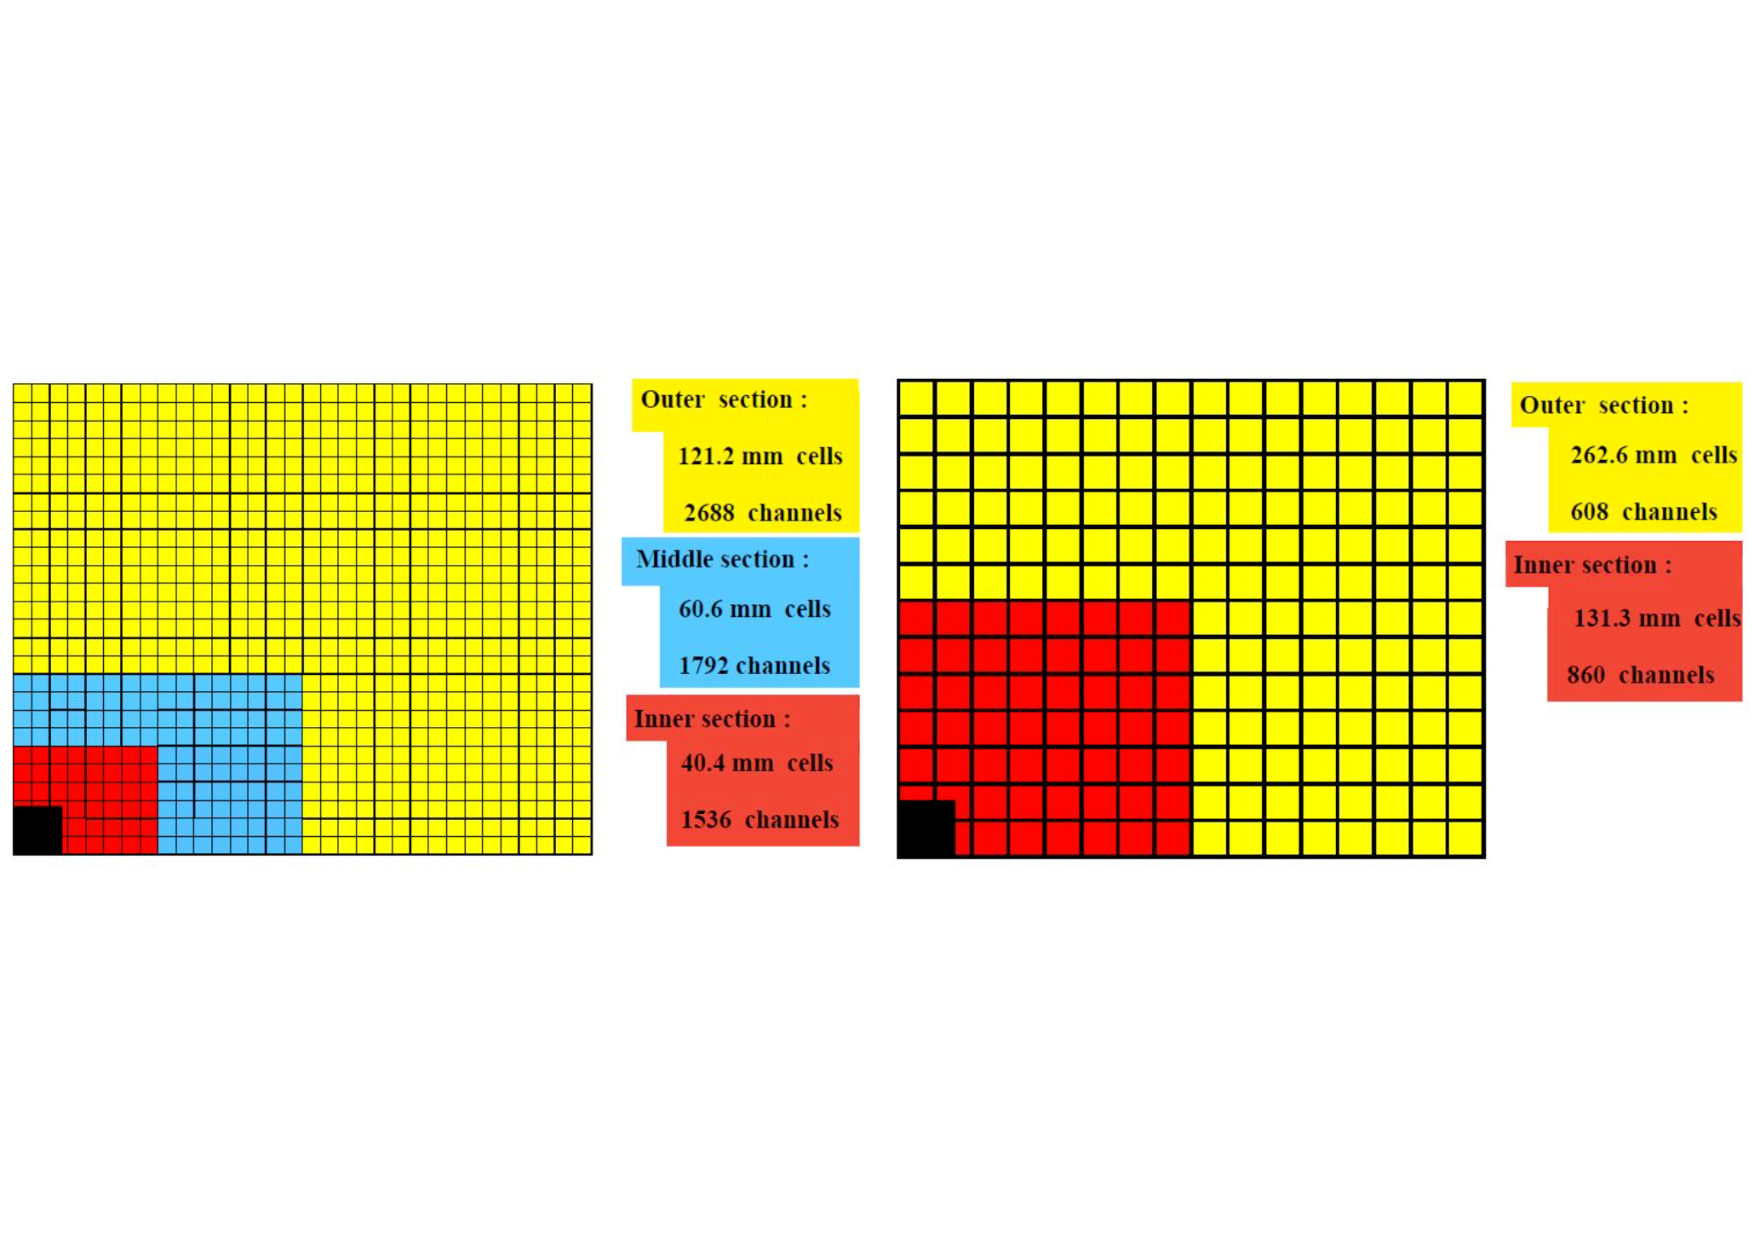
\includegraphics[width=1.0\textwidth]{figures/lhcbCalo.pdf}
  %  \caption{Lateral segmentation of the SPD/PRS and ECAL (left) and
   %   the HCAL (right). One quarter of the detector front face is
  %    shown. In the left figure the cell dimensions are given for the
 %     ECAL.\label{fig:lhcbCalo}}
 % \end{center}
%\end{figure}

\section{Library Approach \label{seq:LA}}
Detailes for this approach may be found elswhere \cite{chepFastSim}.
To reduce the number of parameters in produced response library, the
cell transverse area is divided into small subregions, or "points" and
a library of points is built from simulated incident particles with
fixed values for particle position and azimutal angle. Hence, for a
given particle species only the binnings in energy and incidenсe angle remain. An example of point distribution in the ECAL produced by an incident photon with energy O(1) GeV is shown in Fig. \ref{fig:pointProcessing}, top-left plot, where each square of the grid represents the transverse area of an ECAL cell and the colour scale indicates the deposited energy in MeV.
Then two or more points belonging to the same cell area and with
associated energy below a given threshold may be merged locally to
simplify the collection, i.e. to reduce the number of points stored in
the library. This is exemplified in top-right plot. In the next step
the points are shifted and rotated according to the position of
incidence and azimuthal angle of the particle with respect to the
values for which the library was built. This is a key aspect of the
point library. The collection of points represents a good model of the
shower projection in the transverse plane, so that its shift and
rotation gives a good description of the shower produced by a
translated and rotated incident particle. The rotation of the points
around the position of incidence of the particle is exemplified in
thebottom-left plot. Finally, the calorimeter hits are created by
summing the energies of those transformed points which fall into the
same cell area. This is shown in the bottom-right plot, where the
colour in the central region of the cell indicates the total deposited
energy, in MeV.

\begin{figure}[htb]
  \begin{center}
   \begin{subfigure}[t]{0.4\textwidth}
    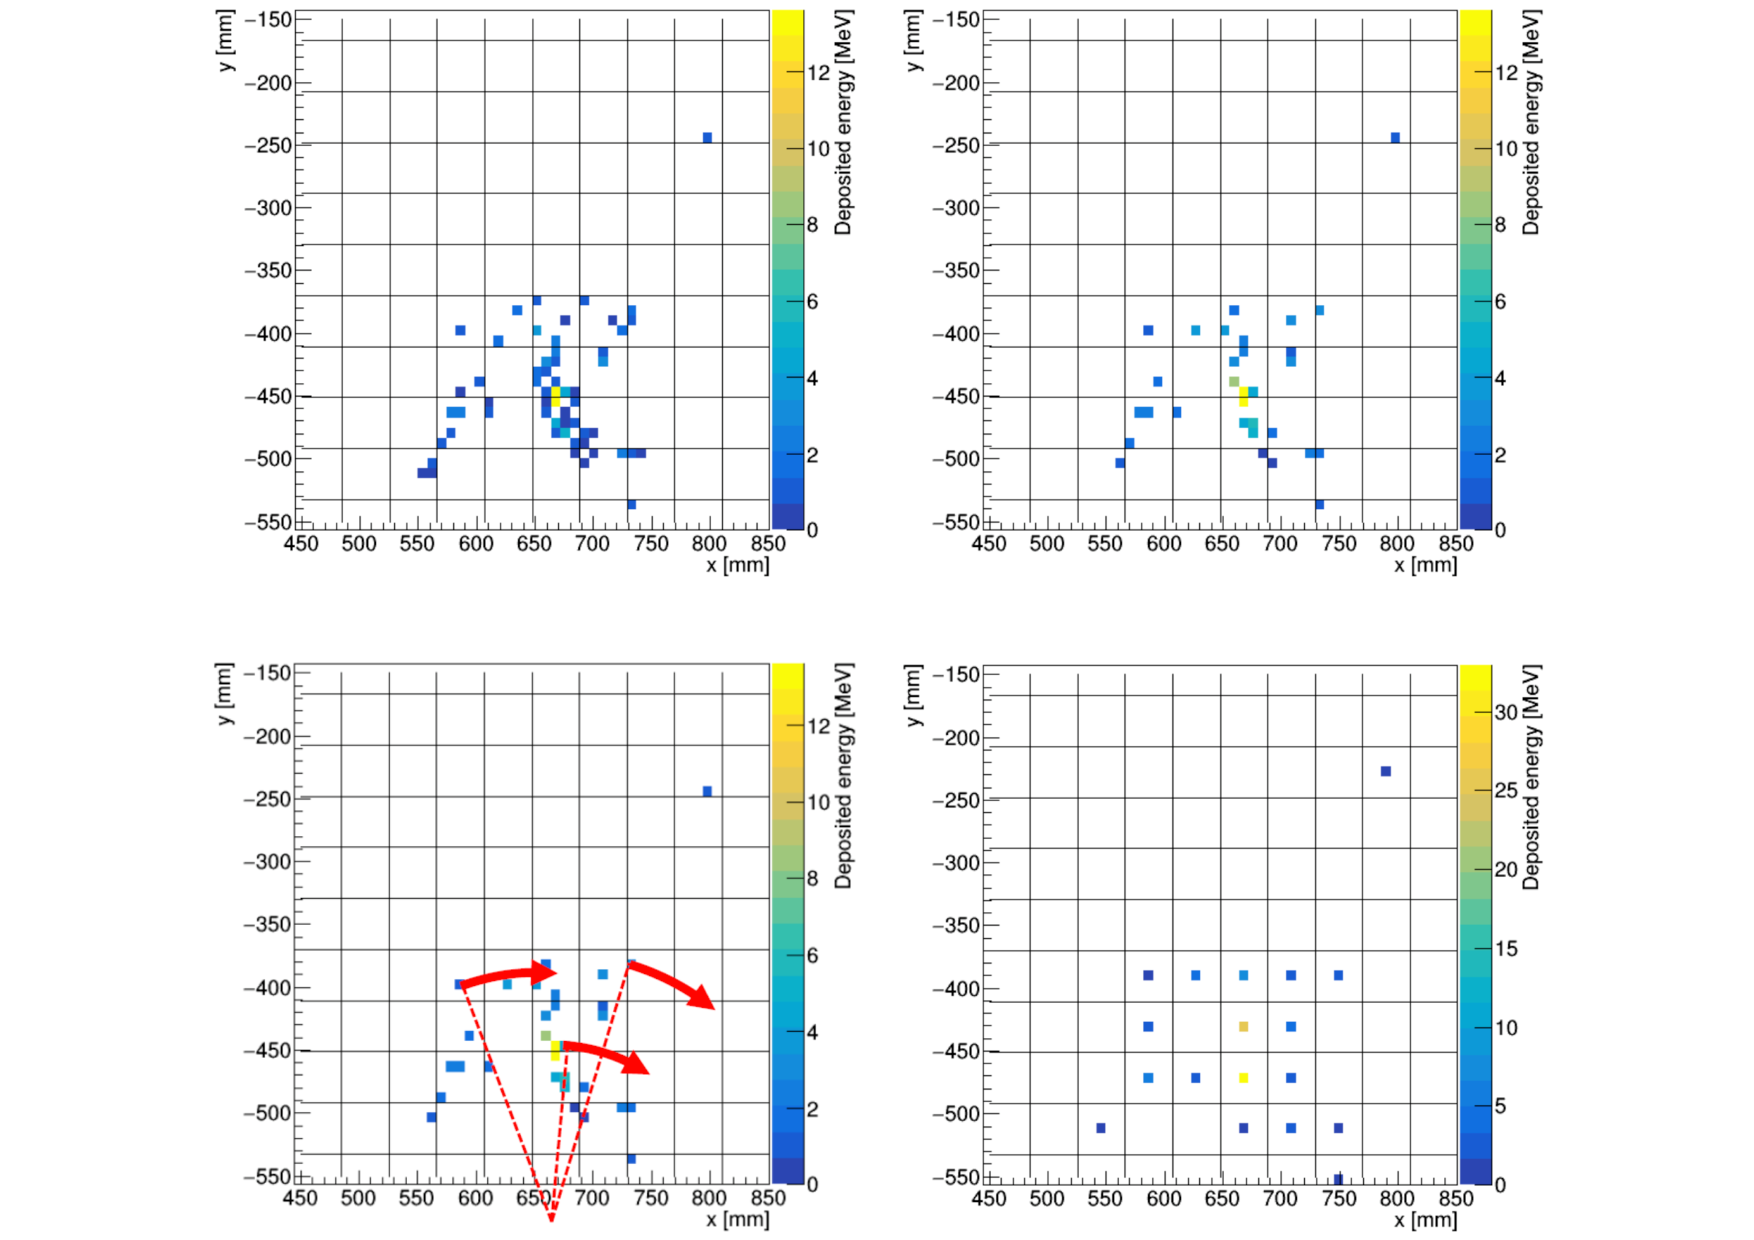
\includegraphics[width=1\textwidth]{figures/pointProcessing.pdf}
    \caption{Schematic illustration of the point library operating
      principle. More details are given in section
      \ref{seq:LA}.\label{fig:pointProcessing}}
  \end{subfigure}
  \hspace{0.04\textwidth}
   \begin{subfigure}[t]{0.52\textwidth}
    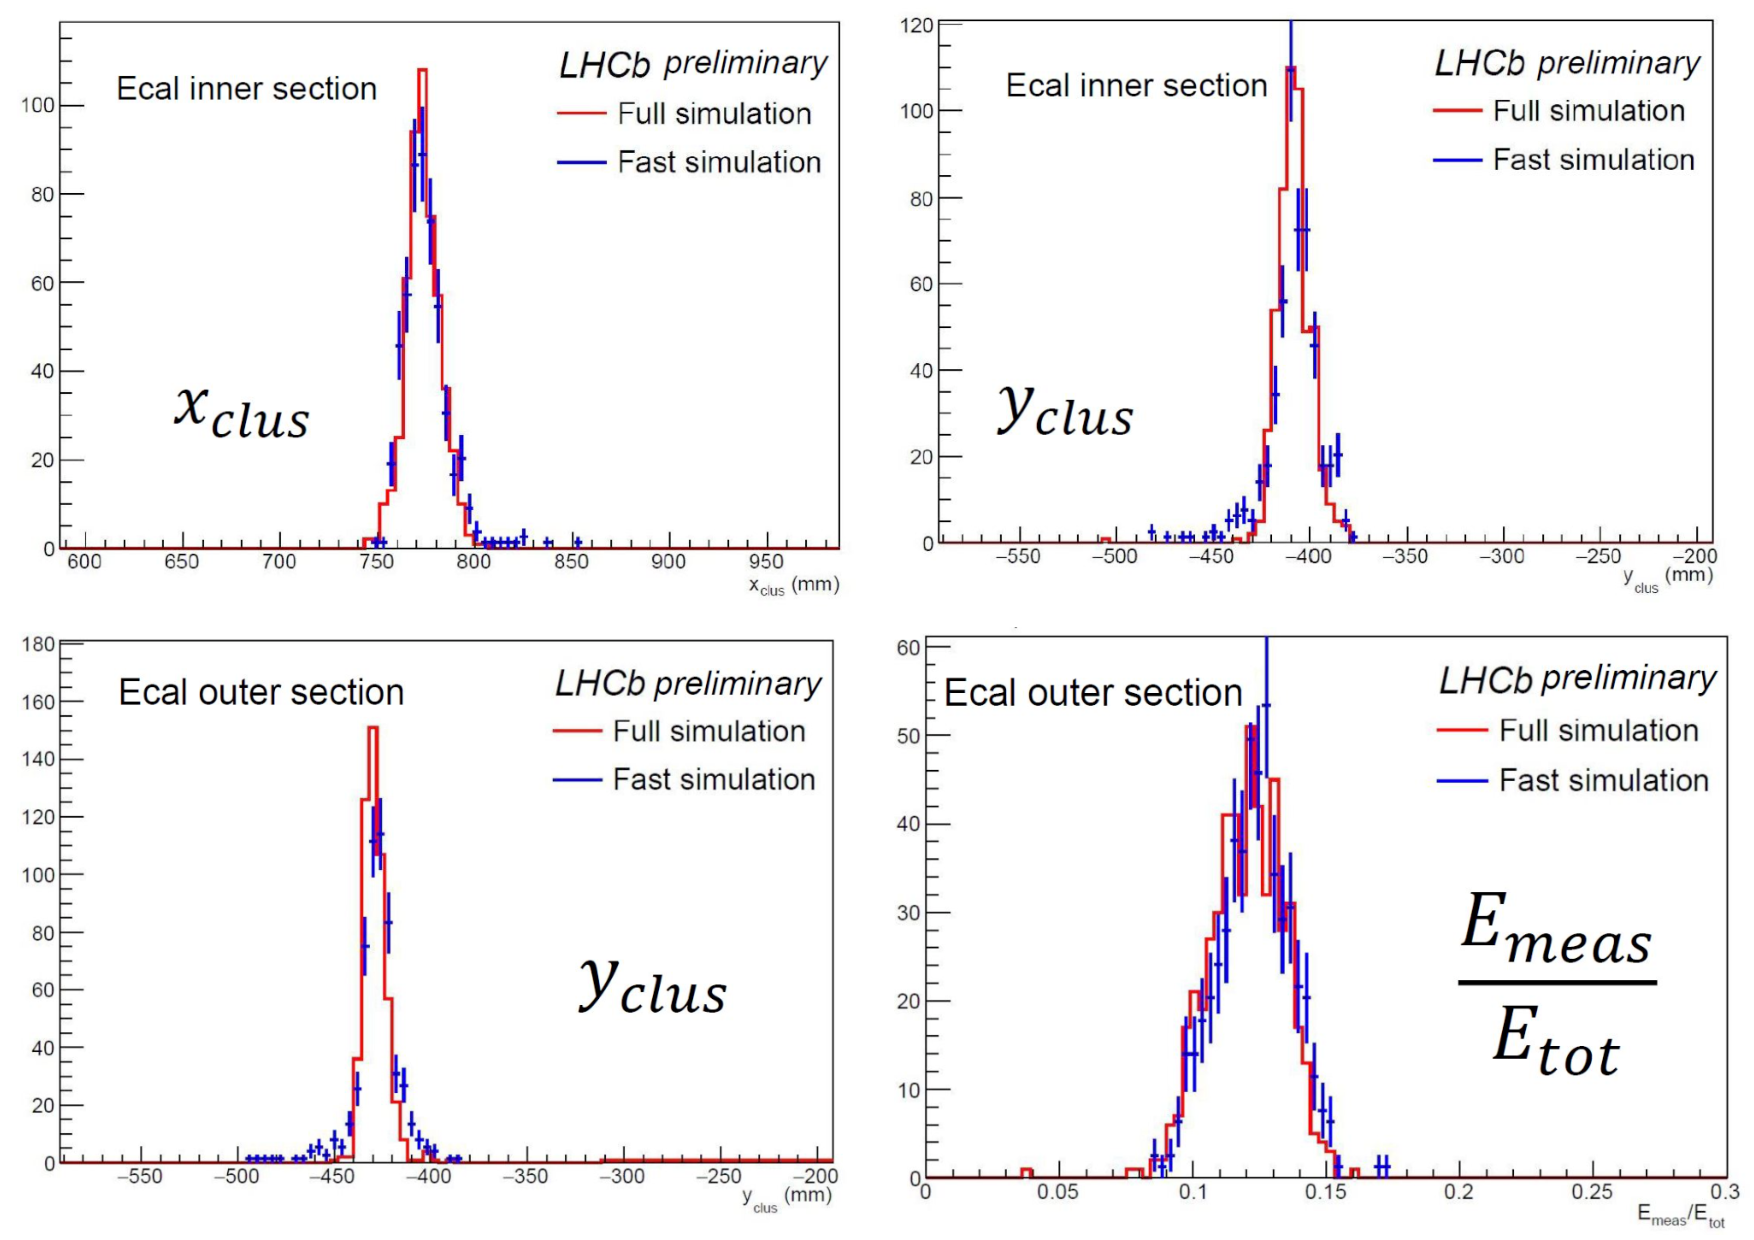
\includegraphics[width=1\textwidth]{figures/showerlibPerf.pdf}
    \caption{Comparison of photons simulated with Geant4 ("Full simulation") and with the point libraries ("Fast simulation") \label{fig:showerlibPerf}}
  \end{subfigure}
  \end{center}
\caption{Library approach.}
\end{figure}

The accuracy of the calorimeter simulation based on point libraries
has been tested through the comparison with detailed simulation using
photons generated at the calorimeter entrance with various energies
and angles of incidence. The coordinates of the hit cluster centre are
defined as weighted with energies mean coordinate of cluster cells. 
The top plots compare the cluster position distributions in the case
where the entrance point of the fully simulated photons coincide with
the one used to build the library, thus only rotation is necessary for
the procedure described above.
The bottom plots compare  distributions for cluster position and
measured energy in the case where the fully simulated photons are
generated in the outer sector. 
In this case the points had to be rotated and then translated but the agreement does not worsen, proving that the idea behind the point library works.

\section {Generative Model Approach}
The idea of this approach  is to treat simulations as a black-box and
replace the traditional Monte Carlo simulation with a method based on
Generative Adversarial Networks \cite{gan}. Wasserstein GAN \cite{wgan}
with gradient penalty are considered to be state-of-the-art technique
for image producing, so a tool based on this particular approach is
used. Architecture of the used Neural Network and details on training
the generative model are present elsewhere \cite{chepGAN}.

After the generative model is built and trained,
we start with comparing original clusters, produced by full Geant4
simulation and clusters generated by the trained model for the same
parameters of the incident particles: the same energy, the same
direction, and the same position on the calorimeter
face. Corresponding images for four arbitrary parameter sets are
presented in Fig. \ref{fig:geant_vs_ours}. These images demonstrate very good visual similarity between simulated and generated clusters.

\begin{figure}
\captionsetup[subfigure]{justification=centering}
  \centering
  \begin{subfigure}{0.24\textwidth}
    \centering
    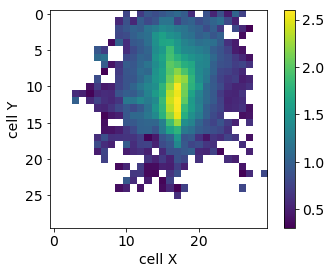
\includegraphics[width=1\textwidth]{figures/1_real.png}
  \end{subfigure}
  \begin{subfigure}{0.24\textwidth}
    \centering
    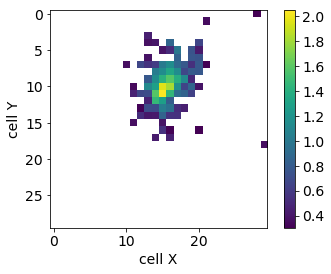
\includegraphics[width=1\textwidth]{figures/2_real.png}
  \end{subfigure}
    \begin{subfigure}{0.24\textwidth}
    \centering
    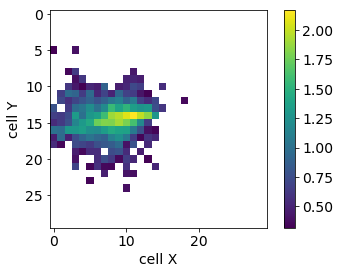
\includegraphics[width=1\textwidth]{figures/3_real.png}
  \end{subfigure}
  \begin{subfigure}{0.24\textwidth}
    \centering
    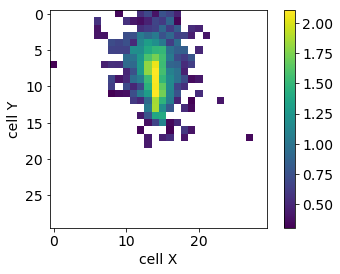
\includegraphics[width=1\textwidth]{figures/4_real.png}
  \end{subfigure}\\
   \begin{subfigure}{0.24\textwidth}
    \centering
    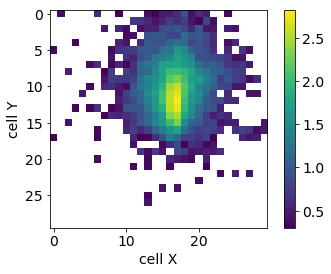
\includegraphics[width=1\textwidth]{figures/1_gen.png}
  \end{subfigure}
  \begin{subfigure}{0.24\textwidth}
    \centering
    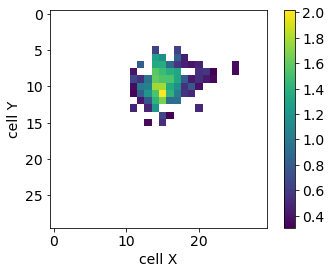
\includegraphics[width=1\textwidth]{figures/2_gen.png}
  \end{subfigure}
    \begin{subfigure}{0.24\textwidth}
    \centering
    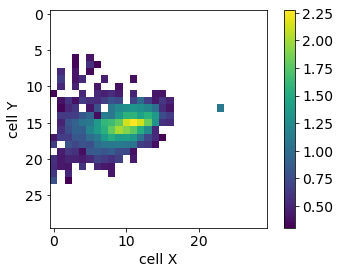
\includegraphics[width=1\textwidth]{figures/3_gen.png}
  \end{subfigure}
  \begin{subfigure}{0.24\textwidth}
    \centering
    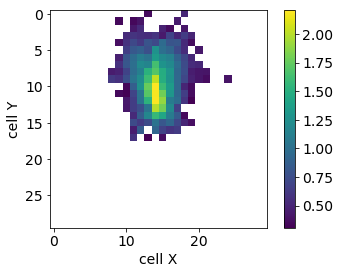
\includegraphics[width=1\textwidth]{figures/4_gen.png}
  \end{subfigure}
   \caption{Showers generated with GEANT4 (first row) and the showers,
    simulated with our model (second row) for three different sets of
    input parameters. Color represents $log_{10}(\frac{E}{MeV})$ for every cell.}
  \label{fig:geant_vs_ours}
\end{figure}

Then we continue with quantitative evaluation of the proposed
simulation method. While generic evaluation methods for generative
models exist, 
here we base our evaluation on
physics-driven similarity metrics. For this presentation we selected
few cluster properties which essentially drive cluster properties used
in the reconstruction of calorimeter objects and following physics
analysis. If initial particle direction is not perpendicular to the
calorimeter face, produced cluster is elongated in that direction. 
Therefore we consider separately cluster width in the direction of the
initial particle and in the transverse direction. 
Spatial resolution, that is the distance between center mass of the
cluster and the initial track projection to the shower max depth, is
another important characteristics affecting physics properties of the
cluster.
 Cluster sparsity, that is the fraction of cells with energies above
 some threshold, reflects marginal low energy properties of the
 generated clusters. 
These characteristics are presented in Fig. \ref{fig:ganquality}.

\begin{figure}[htb]
\begin{center}
 \begin{subfigure}[t]{0.3\textwidth}
      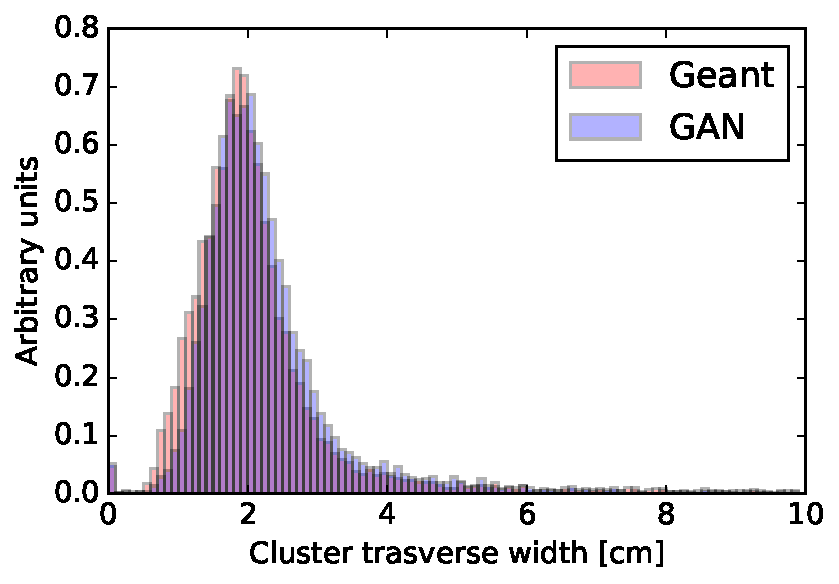
\includegraphics[width=1\textwidth]{figures/width_trans.pdf}
    \caption{The transverse width of real and generated clusters}
  \end{subfigure}\hspace{0.2\textwidth}
 \begin{subfigure}[t]{0.3\textwidth}
    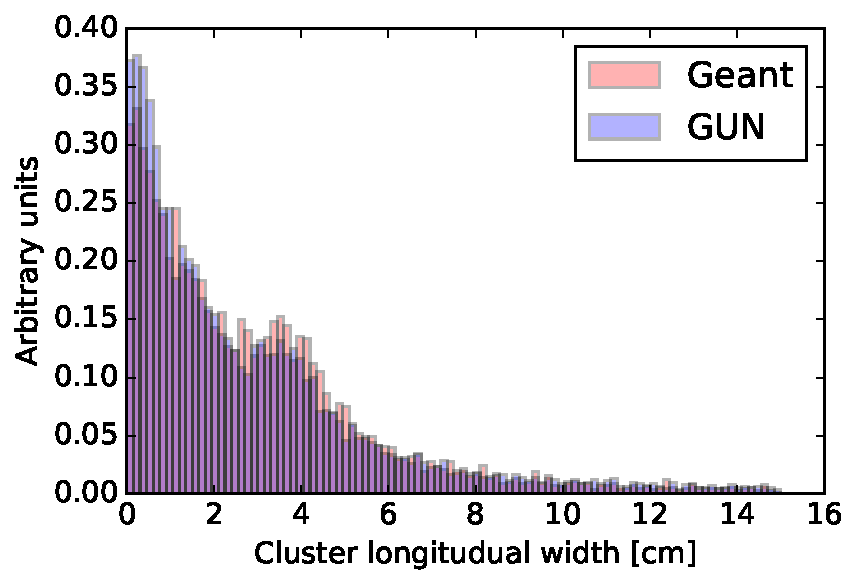
\includegraphics[width=1\textwidth]{figures/width_long.pdf}
    \caption{The longitudinal width of real and generated clusters}
  \end{subfigure}
\end{center}
\begin{center}
  \begin{subfigure}[t]{0.3\textwidth}
    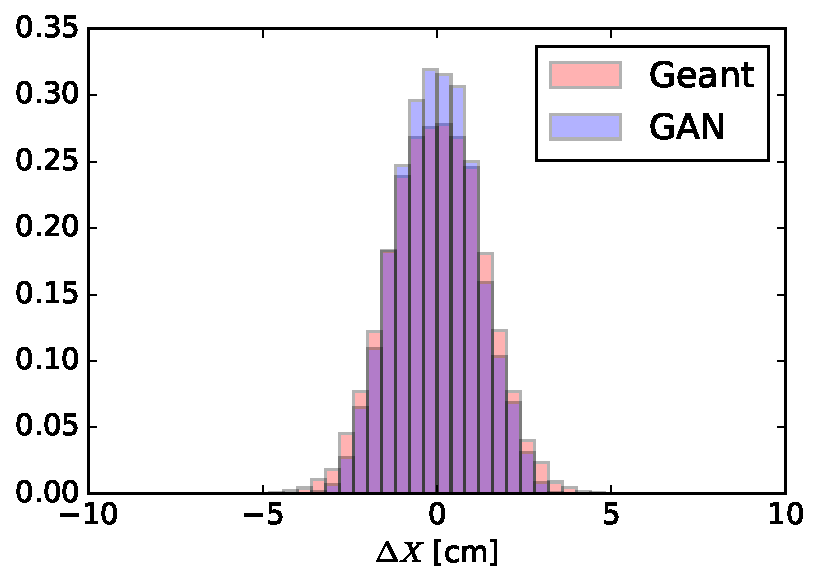
\includegraphics[width=1\textwidth]{figures/deltaX.pdf}
    \caption{$\Delta X$ between cluster center of mass and the true particle coordinate}
  \end{subfigure}\hspace{0.2\textwidth}
  \begin{subfigure}[t]{0.3\textwidth}
    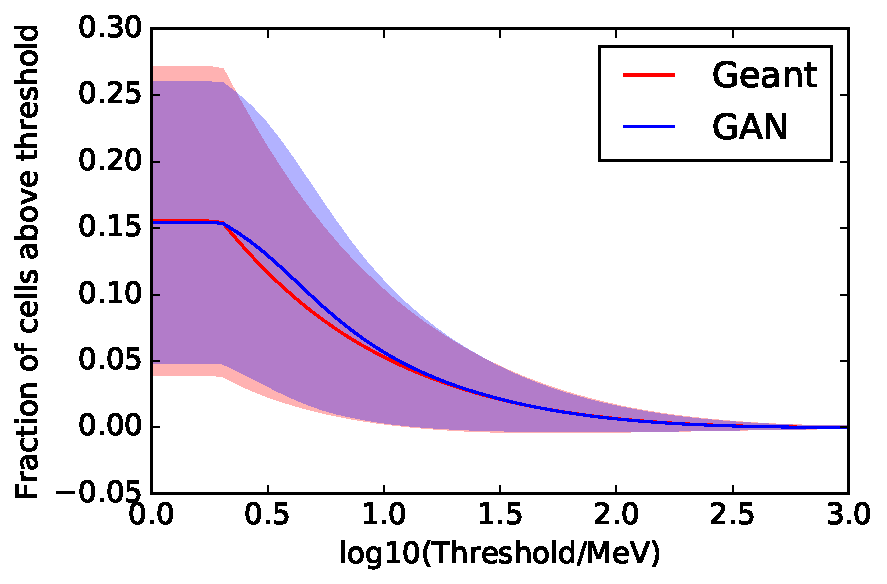
\includegraphics[width=1\textwidth]{figures/sparsity.pdf}
    \caption{The sparsity of real and generated clusters}
  \end{subfigure}
\end{center}
 \caption{Generated images quality evaluation including described
   physical characteristics.}\label{fig:ganquality}
\end{figure}


\section {Conclusions}
In LHCb there is an ongoing effort to develop fast simulation
alternatives to the nominal detector simulation to face the current
and future limitations of CPU resources with respect to the size of
the necessary simulated samples. In the detailed simulation based on
Geant4 more than 50\% of the CPU time is spent in the calorimeter
system. We use different approaches to develop  faster simulation of
the calorimeter.
Both library and generative model approaches are encouraging in terms
of  time gain and simulation accuracy.
The use of a point library as opposed to a more standard cell hit library allows to significantly improve the output accuracy for the same size of the library.
We also prove  that Generative Adversarial Networks are a good
candidate for fast simulating of high granularity detectors typically
studied for the next generation accelerators. 
We have successfully generated images of shower energy deposition with
a condition on the particle parameters such as the momentum and the
coordinate 
using modern generative deep neural network techniques.

%\bibliography{ichep18_ratnikov}

\begin{thebibliography}{99}
\bibitem{LHCbCompUpgTDR}LHCb collaboration, LHCb Upgrade Software and
  Computing Technical Design Report, CERN-LHCC-2018-007, LHCb-TDR-017.
\bibitem{geant4}S.Agostinelli et al.,(Geant4 Collaboration), Geant4:
  Asimulation toolkit,Nucl.Instrum. Methods Phys. Res., Sect. A 506, 250 (2003); J. Allison et al., (Geant4
  Collaboration), IEEE Trans. Nucl. Sci. 53, 270 (2006).
\bibitem{LHCb}LHCb collaboration, A. A. Alves Jr. et al., The LHCb detector at the LHC, JINST 3
(2008) S08005.
\bibitem{chepFastSim}M.Rama and G.Vitali (LHCb collaboration),
  Calorimeter fast simulation based on hit libraries in the LHCb Gauss
  framework, procedengs of CHEP2018 conference, to be published in the
  EPJ Web of Conferences.
\bibitem{gan}I. Goodfellow, J. Pouget-Abadie, M. Mirza, B. Xu, D. Warde-Farley, S. Ozair,
A. Courville, Y. Bengio, Generative adversarial nets, in Advances in neural information
processing systems (2014), pp. 2672–2680.
\bibitem{wgan}T.C. Wang, M.Y. Liu, J.Y. Zhu, G. Liu, A. Tao, J. Kautz, B. Catanzaro, arXiv preprint
arXiv:1808.06601 (2018).
\bibitem{chepGAN}V.Chekalina et al., Generative Models for Fast Calorimeter Simulation: LHCb case, procedengs of CHEP2018 conference, to be published in the
  EPJ Web of Conferences.
\end{thebibliography}

\end{document}
